% XXX Jedes Jahr Professoren-Texte aktualisieren!
\section[Eure Profs stellen sich vor]{Eure Professoren stellen sich vor}
\textbf{Auf den folgenden zwei Seiten stellen sich eure beiden Professoren vor.
    Sie werden gemeinsam die "Physik~1" bis "Physik~3" lesen.
    Prof.\ Linz wird sich dabei um die theoretischen und Prof.\ Krenner um die experimentellen Aspekte des Studiums kümmern.
    Zudem stellt sich Prof.\ Wulkenhaar vor, der die Vorlesungen "Mathematik für Studierende der Physik" halten wird (ebenfalls über drei Semester).
	Da diese drei Professoren euch eine Zeit lang begleiten werden, ist es durchaus mal interessant zu wissen, was sie gemacht haben, bevor sie an die Uni Münster kamen, und wie ihre aktuelle Forschung aussieht.}

\begin{multicols}{2}
\begin{center}
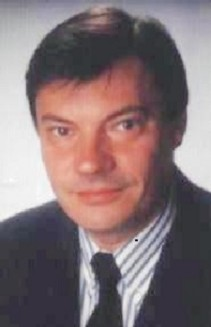
\includegraphics[width=0.71\columnwidth]{res/vorstellungsfotos/linz.jpg}\\
Prof.\ Dr.\ Stefan J.~Linz\\
Institut für Theoretische Physik
\end{center}

Ich freue mich darauf, in den nächsten drei Semestern den theoretischen Teil des integrierten Kurses zu lesen. Dabei möchte ich Ihnen nicht nur die theoretischen Grundlagen der Klassischen Physik vermitteln, sondern Sie auch in die grundlegenden Konzepte und Denkweisen der
theoretischen Physik einführen und Ihnen die Effektivität und Eleganz einer mathematisch formulierten Naturbeschreibung näher bringen. Meine Grundausbildung als Physiker habe ich an der Universität des Saarlandes in Saarbrücken erhalten und dort auch 1989 promoviert. Daran schloss sich ein mehrjähriger Auslandsaufenthalt in den USA an, als Postdoctoral Fellow bei der Woods Hole Oceanographic Institution (WHOI) und danach als Research Associate im Department of Applied Mathematics der Northwestern University in Evanston bei Chicago. Nach Rückkehr nach Deutschland arbeitete ich als wissenschaftlicher Assistent, später als Oberassistent im Institut für Physik an der Universität Augsburg, wo ich mich 1997 habilitierte und zum Privatdozenten ernannt wurde. 2002 folgte ich einem Ruf auf eine Professur für Theoretische Physik an der WWU Münster.

Forschungsschwerpunkt meiner Arbeitsgruppe ist Theorie komplexer Systeme, insbesondere die Modellierung und theoretische Analyse zeitlicher bzw.\ raumzeitlicher Dynamik in Systemen, die spontan durch das Wechselspiel von Nichtgleichgewicht, Nichtlinearität und Dissipation entstehen kann. Physikalisch stehen dabei Depositions- und Erosionsphänomene, die Dynamik granularer Materie und komplexer Fluide sowie mathematische Aspekte der Theorie chaotischer Systeme im Vordergrund.

\end{multicols}

\begin{center}
    \fibelimgtext{
	\includegraphics[width=0.7\textwidth]{res/xkcd/895_teaching_physics.png}
    }{\url{https://xkcd.com/895}}
\end{center}

\newpage

\begin{multicols}{2}
\begin{center}
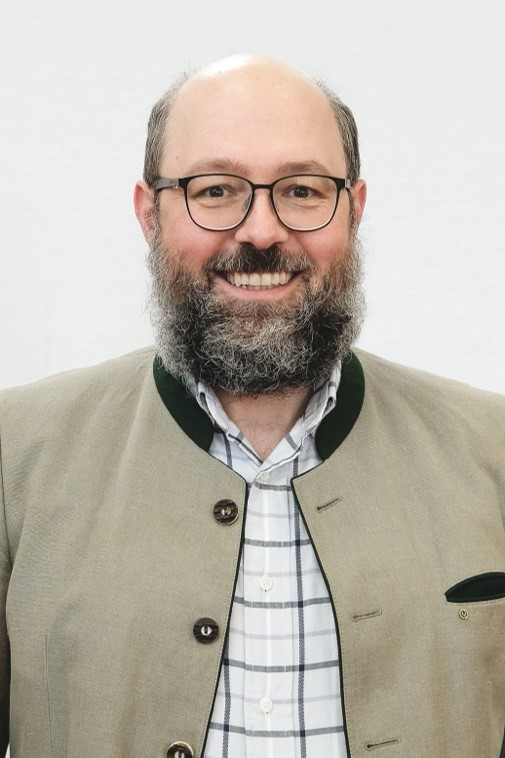
\includegraphics[width=0.8\columnwidth]{res/vorstellungsfotos/krenner.jpg}\\
\smallskip
Prof.\ Dr.\ Hubert Krenner\\
Physikalisches Institut
\end{center}

Herzlich Willkommen an der Universität Münster! Ich freue mich sehr, dass Sie sich für unseren Physik Bachelor-Studiengang entschieden haben – eine gute Wahl. In den nächsten drei Semestern werden wir uns zusammen im Rahmen der Physik~1-3 Vorlesung mit Grundlagen der Experimentalphysik beschäftigen. Auch für mich ist diese Vorlesung meine erste, die ich hier an der Universität Münster halten darf. Ich bin vergangenen Sommer von aus dem Süden nach 12 Jahren als Nachwuchsgruppenleiter und später Professor von der Universität Augsburg, an der ich seit 2014 Professor war, nach Münster gewechselt. Daher bin ich – zwar unter etwas anderen Vorzeichen – ins erste Semester gestartet. Mein Physik-Studium habe ich 2002 an der TU München abgeschlossen, an der ich dann ebenfalls eine Doktorarbeit angeschlossen habe. Im Anschluss habe ich mit einem Forschungsstipendium zwei Jahre an der University of California in Santa Barbara geforscht bevor ich dann nach Augsburg gewechselt bin.

In die Experimentalphysik starten wir mit den ganz fundamentalen Prinzipien der Newtonschen Mechanik, die manche von Ihnen vielleicht schon aus der Schule kennen. Eng verzahnt mit der Theoretischen Physik, die Sie bei Prof.\ Stefan Linz hören werden, spannen wir einen weiten Bogen durch die wichtigsten Teilbereiche der Physik wie der Thermodynamik oder dem Elektromagnetismus. Am Ende dieser drei Semester werden Sie das Rüstzeug besitzen, sich in den vielen Facetten und Gebiete der modernen Physik zurecht zu finden und diese zu erschließen, insbesondere die, in denen hier an der Universität Münster Spitzenforschung betrieben wird.

In meiner Arbeitsgruppe, die gerade dabei ist von Augsburg nach Münster umzuziehen, befassen wir uns mit „Nanoerdbeben“, sogenannten akustischen Oberflächenwellen. Diese sind ein Paradebeispiel eines Wellenphänomens, welche wir auch in unserer Vorlesung genau untersuchen und verstehen werden. Diese Tausendsassa der Nanophysik verwenden wir in der Forschung, um die elektrischen und optischen Eigenschaften von neuen Materialien zu enträtseln oder sogar einzelne Lichtquanten -- Photonen -- mit ungeahnter Präzision zu kontrollieren. Aber mehr dazu erfahren Sie von uns, wenn Sie sich auf dem Bachelor-Mastertag nach einem spannenden Thema für Ihre Abschlussarbeit umsehen. :)

Ich wünsche Ihnen ganz herzlich einen guten Start in Ihr Studium, viele gute neue Freunde, tolle Erfahrungen und Eindrücke, viel Erfolg und ganz viel Spaß an der Physik!

\begin{center}
\includegraphics[width=0.85\columnwidth]{private/res/comics/manchmal_edited.jpg}\\
{\footnotesize 
S.~Harris – sciencecartoonsplus.com}
\end{center}

\end{multicols}

\vfill

\newpage

\begin{multicols}{2}
\begin{center}
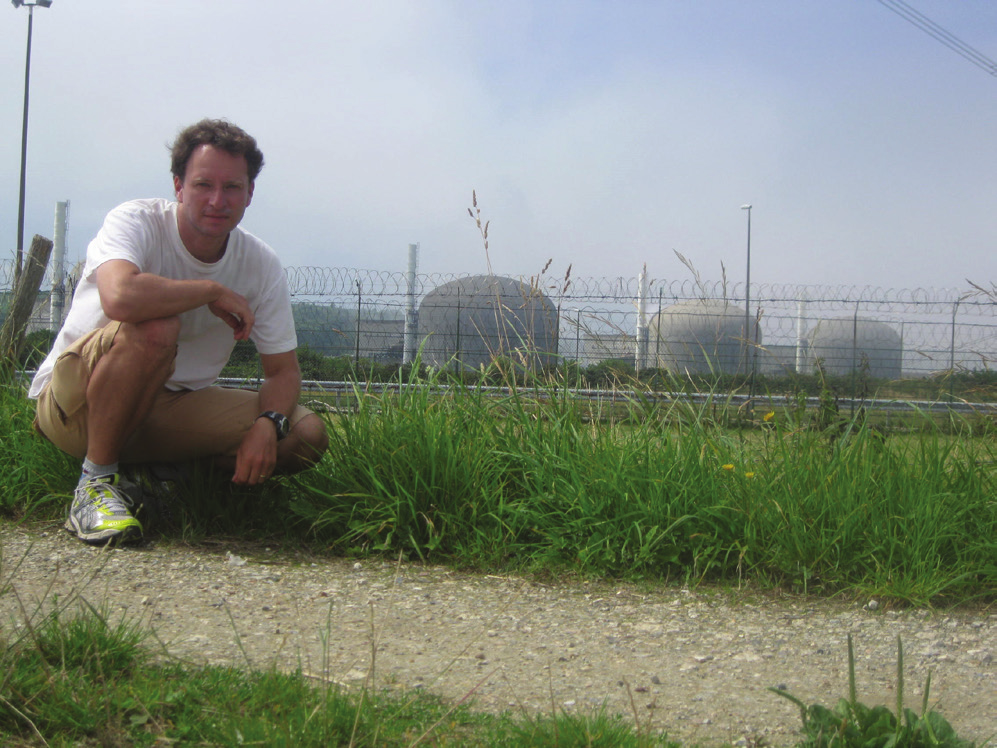
\includegraphics[width=0.9\columnwidth]{res/vorstellungsfotos/wulkenhaar.png}\\
Prof.\ Dr.\ Raimar Wulkenhaar\\
Mathematisches Institut
\end{center}

Ich bin von der Ausbildung her Physiker, arbeite im Grenzgebiet zwischen Mathematik und Physik und bin seit 2005 Professor für Reine Mathematik am Fachbereich Mathematik und Informatik der WWU.

Die Vorlesung "Mathematik für Studierende der Physik" wird traditionell vom Mathematischen Institut veranstaltet. Ich selbst werde den Zyklus zum 9.~Mal halten. Es ist aus meiner Sicht eine schöne Vorlesung; mir ist aber klar, dass die meisten Studierenden das anders sehen.

Auch wenn der Stoff durchaus umfangreich ist, können wir nur einen kleinen Teil dessen behandeln, was die Physik benötigt. Es geht in der Vorlesung nicht um die Bereitstellung von Rechenwerkzeugen für die Physik; das bekommen Sie nebenbei in den Physikvorlesungen geliefert. Es geht in der Mathematik darum zu verstehen, weshalb diese Rechenwerkzeuge so und nicht anders funktionieren. Der Einstieg in die Denkweise der Mathematik ist für viele nicht leicht. Erst im Lauf der Zeit entsteht rückblickend ein gewisses Verständnis für die tiefliegenden Strukturen und Zusammenhänge der Mathematik. Im Idealfall gelangen Sie so zu einer soliden Grundlage, mit der Sie die Rechenwerkzeuge der Physik nicht nur verstehend nutzen, sondern kreativ weiterentwickeln können.


\[
\resizebox{0.45\hsize}{!}{$\displaystyle\sum_{n = 1}^\infty \frac{1}{n^2} = \frac{\pi^2}{6}$}
\]

Nun noch einige Informationen zu mir. Nach Physikistudium an der Universität Leipzig mit Abschluss als Diplomphysiker. 1994 habe ich in Leipzig auch meine Doktorarbeit geschrieben und 1997 verteidigt. Dabei ging es um die Formulierung von Modellen der Teilchenphysik im Rahmen der nichtkommutativen Geometrie. Die Ergebnisse sind rückblickend völlig unwichtig, sie haben mich aber 1998/1999 als DAAD-Postdoc nach Marseille gebracht.

Ich habe am Centre de Physique Theorique in Marseille mein Arbeitsgebiet gefunden, die Quantenfeldtheorie auf nichtkommutativen Geometrien. Vereinfacht gesagt geht es um die Frage (und ihre Konsequenzen), ob man auf beliebig kleinen Längenskalen, sagen wir $10^{-80}$\,m, noch Physik betreiben kann. Es gibt gute Gründe anzunehmen, dass das unmöglich ist, und entsprechend sollte zur Formulierung physikalischer Gesetze eine Geometrie benutzt werden, in der $10^{-80}$\,m ebenfalls sinnlos sind. Diese Nichtkommutative Geometrie wird in einer Sprache analog zur Quantenphysik beschrieben.

Seit Marseille, vor allem aber seit meiner zweiten Postdoc-Station 2000/2001 an der Universität Wien, arbeite ich an quantenfeldtheoretischen Modellen auf einer besonders einfachen nichtkommutativen Geometrie. Während meines dritten Postdoc-Aufenthalts 2002/2005 am Max- Planck-Institut für Mathematik in den Naturwissenschaften in Leipzig konnte ich mit meinem Kollegen aus Wien zusammen eine größere Hürde beseitigen. Die mathematisch rigorose Konstruktion einer 4-dimensionalen Quantenfeldtheorie auf einer nichtkommutativen Geometrie konnten wir inzwischen abschließen. Etwas analoges ist in der üblichen kommutativen Geometrie bisher nicht geglückt. Es resultierten spannende Fragen, an denen ich seitdem arbeite.

\begin{center}
\includegraphics[width=0.85\columnwidth]{private/res/comics/calvin_mathe.pdf}
\end{center}
\end{multicols}
